\documentclass[10,portrait]{article}
\usepackage{lmodern}
\usepackage{amssymb,amsmath}
\usepackage{ifxetex,ifluatex}
\usepackage{fixltx2e} % provides \textsubscript
\ifnum 0\ifxetex 1\fi\ifluatex 1\fi=0 % if pdftex
  \usepackage[T1]{fontenc}
  \usepackage[utf8]{inputenc}
\else % if luatex or xelatex
  \ifxetex
    \usepackage{mathspec}
  \else
    \usepackage{fontspec}
  \fi
  \defaultfontfeatures{Ligatures=TeX,Scale=MatchLowercase}
\fi
% use upquote if available, for straight quotes in verbatim environments
\IfFileExists{upquote.sty}{\usepackage{upquote}}{}
% use microtype if available
\IfFileExists{microtype.sty}{%
\usepackage[]{microtype}
\UseMicrotypeSet[protrusion]{basicmath} % disable protrusion for tt fonts
}{}
\PassOptionsToPackage{hyphens}{url} % url is loaded by hyperref
\usepackage[unicode=true]{hyperref}
\PassOptionsToPackage{usenames,dvipsnames}{color} % color is loaded by hyperref
\hypersetup{
            pdftitle={The Life of Eli},
            colorlinks=true,
            linkcolor=pink,
            citecolor=red,
            urlcolor=blue,
            breaklinks=true}
\urlstyle{same}  % don't use monospace font for urls
\usepackage[margin=1in]{geometry}
\usepackage[]{biblatex}
\usepackage{color}
\usepackage{fancyvrb}
\newcommand{\VerbBar}{|}
\newcommand{\VERB}{\Verb[commandchars=\\\{\}]}
\DefineVerbatimEnvironment{Highlighting}{Verbatim}{commandchars=\\\{\}}
% Add ',fontsize=\small' for more characters per line
\usepackage{framed}
\definecolor{shadecolor}{RGB}{248,248,248}
\newenvironment{Shaded}{\begin{snugshade}}{\end{snugshade}}
\newcommand{\KeywordTok}[1]{\textcolor[rgb]{0.13,0.29,0.53}{\textbf{#1}}}
\newcommand{\DataTypeTok}[1]{\textcolor[rgb]{0.13,0.29,0.53}{#1}}
\newcommand{\DecValTok}[1]{\textcolor[rgb]{0.00,0.00,0.81}{#1}}
\newcommand{\BaseNTok}[1]{\textcolor[rgb]{0.00,0.00,0.81}{#1}}
\newcommand{\FloatTok}[1]{\textcolor[rgb]{0.00,0.00,0.81}{#1}}
\newcommand{\ConstantTok}[1]{\textcolor[rgb]{0.00,0.00,0.00}{#1}}
\newcommand{\CharTok}[1]{\textcolor[rgb]{0.31,0.60,0.02}{#1}}
\newcommand{\SpecialCharTok}[1]{\textcolor[rgb]{0.00,0.00,0.00}{#1}}
\newcommand{\StringTok}[1]{\textcolor[rgb]{0.31,0.60,0.02}{#1}}
\newcommand{\VerbatimStringTok}[1]{\textcolor[rgb]{0.31,0.60,0.02}{#1}}
\newcommand{\SpecialStringTok}[1]{\textcolor[rgb]{0.31,0.60,0.02}{#1}}
\newcommand{\ImportTok}[1]{#1}
\newcommand{\CommentTok}[1]{\textcolor[rgb]{0.56,0.35,0.01}{\textit{#1}}}
\newcommand{\DocumentationTok}[1]{\textcolor[rgb]{0.56,0.35,0.01}{\textbf{\textit{#1}}}}
\newcommand{\AnnotationTok}[1]{\textcolor[rgb]{0.56,0.35,0.01}{\textbf{\textit{#1}}}}
\newcommand{\CommentVarTok}[1]{\textcolor[rgb]{0.56,0.35,0.01}{\textbf{\textit{#1}}}}
\newcommand{\OtherTok}[1]{\textcolor[rgb]{0.56,0.35,0.01}{#1}}
\newcommand{\FunctionTok}[1]{\textcolor[rgb]{0.00,0.00,0.00}{#1}}
\newcommand{\VariableTok}[1]{\textcolor[rgb]{0.00,0.00,0.00}{#1}}
\newcommand{\ControlFlowTok}[1]{\textcolor[rgb]{0.13,0.29,0.53}{\textbf{#1}}}
\newcommand{\OperatorTok}[1]{\textcolor[rgb]{0.81,0.36,0.00}{\textbf{#1}}}
\newcommand{\BuiltInTok}[1]{#1}
\newcommand{\ExtensionTok}[1]{#1}
\newcommand{\PreprocessorTok}[1]{\textcolor[rgb]{0.56,0.35,0.01}{\textit{#1}}}
\newcommand{\AttributeTok}[1]{\textcolor[rgb]{0.77,0.63,0.00}{#1}}
\newcommand{\RegionMarkerTok}[1]{#1}
\newcommand{\InformationTok}[1]{\textcolor[rgb]{0.56,0.35,0.01}{\textbf{\textit{#1}}}}
\newcommand{\WarningTok}[1]{\textcolor[rgb]{0.56,0.35,0.01}{\textbf{\textit{#1}}}}
\newcommand{\AlertTok}[1]{\textcolor[rgb]{0.94,0.16,0.16}{#1}}
\newcommand{\ErrorTok}[1]{\textcolor[rgb]{0.64,0.00,0.00}{\textbf{#1}}}
\newcommand{\NormalTok}[1]{#1}
\usepackage{graphicx,grffile}
\makeatletter
\def\maxwidth{\ifdim\Gin@nat@width>\linewidth\linewidth\else\Gin@nat@width\fi}
\def\maxheight{\ifdim\Gin@nat@height>\textheight\textheight\else\Gin@nat@height\fi}
\makeatother
% Scale images if necessary, so that they will not overflow the page
% margins by default, and it is still possible to overwrite the defaults
% using explicit options in \includegraphics[width, height, ...]{}
\setkeys{Gin}{width=\maxwidth,height=\maxheight,keepaspectratio}
\usepackage[normalem]{ulem}
% avoid problems with \sout in headers with hyperref:
\pdfstringdefDisableCommands{\renewcommand{\sout}{}}
\IfFileExists{parskip.sty}{%
\usepackage{parskip}
}{% else
\setlength{\parindent}{0pt}
\setlength{\parskip}{6pt plus 2pt minus 1pt}
}
\setlength{\emergencystretch}{3em}  % prevent overfull lines
\providecommand{\tightlist}{%
  \setlength{\itemsep}{0pt}\setlength{\parskip}{0pt}}
\setcounter{secnumdepth}{0}
% Redefines (sub)paragraphs to behave more like sections
\ifx\paragraph\undefined\else
\let\oldparagraph\paragraph
\renewcommand{\paragraph}[1]{\oldparagraph{#1}\mbox{}}
\fi
\ifx\subparagraph\undefined\else
\let\oldsubparagraph\subparagraph
\renewcommand{\subparagraph}[1]{\oldsubparagraph{#1}\mbox{}}
\fi

% set default figure placement to htbp
\makeatletter
\def\fps@figure{htbp}
\makeatother


\title{The Life of Eli}
\author{Matthew Malishev\textsuperscript{1}*\\
\emph{\textsuperscript{1} Department of Biology, Emory University, 1510
Clifton Road NE, Atlanta, GA, USA, 30322}}
\date{}

\begin{document}
\maketitle

{
\hypersetup{linkcolor=black}
\setcounter{tocdepth}{4}
\tableofcontents
}
~

Date: 2018-08-18\\
R version: 3.5.0\\
*Corresponding author:
\href{mailto:matthew.malishev@gmail.com}{\nolinkurl{matthew.malishev@gmail.com}}\\
This document can be found at
\url{https://github.com/darwinanddavis/Eli}

\newpage  

\subsection{Overview}\label{overview}

Activity data for Eli for his first year, including time spent feeding,
sleeping, in leisure and values for growth and other behavoural traits.

~

\textbf{TO DO}\\
* \sout{separate activity states}\\
* separate hour and mins, then convert time to hours

\subsubsection{Install dependencies}\label{install-dependencies}

\begin{Shaded}
\begin{Highlighting}[]
\NormalTok{packages <-}\StringTok{ }\KeywordTok{c}\NormalTok{(}\StringTok{"stringi"}\NormalTok{,}\StringTok{"tidyr"}\NormalTok{,}\StringTok{"sp"}\NormalTok{,}\StringTok{"RColorBrewer"}\NormalTok{,}\StringTok{"ggplot2"}\NormalTok{,}\StringTok{"ggthemes"}\NormalTok{)   }
\ControlFlowTok{if}\NormalTok{ (}\KeywordTok{require}\NormalTok{(packages)) \{}
    \KeywordTok{install.packages}\NormalTok{(packages,}\DataTypeTok{dependencies =}\NormalTok{ T)}
    \KeywordTok{require}\NormalTok{(packages)}
\NormalTok{\}}
\KeywordTok{lapply}\NormalTok{(packages,library,}\DataTypeTok{character.only=}\NormalTok{T)}
\end{Highlighting}
\end{Shaded}

\subsubsection{Set plotting function}\label{set-plotting-function}

\begin{Shaded}
\begin{Highlighting}[]
\CommentTok{# plotting function (plot for MS or not, set bg color, set color palette from RColorBrewer, set alpha value for transperancy) }
\NormalTok{plot_it <-}\StringTok{ }\ControlFlowTok{function}\NormalTok{(manuscript,bg,cp,alpha,family)\{ }
  \KeywordTok{graphics.off}\NormalTok{()}
  \ControlFlowTok{if}\NormalTok{(manuscript}\OperatorTok{==}\DecValTok{0}\NormalTok{)\{}
    \ControlFlowTok{if}\NormalTok{(bg}\OperatorTok{==}\StringTok{"black"}\NormalTok{)\{}
\NormalTok{      colvec<-}\KeywordTok{magma}\NormalTok{(}\DecValTok{200}\NormalTok{,}\DecValTok{1}\NormalTok{)}
      \KeywordTok{par}\NormalTok{(}\DataTypeTok{bg =}\NormalTok{ colvec[}\DecValTok{1}\NormalTok{],}\DataTypeTok{col.axis=}\StringTok{"white"}\NormalTok{,}\DataTypeTok{col.lab=}\StringTok{"white"}\NormalTok{,}\DataTypeTok{col.main=}\StringTok{"white"}\NormalTok{,}
          \DataTypeTok{fg=}\StringTok{"white"}\NormalTok{,}\DataTypeTok{bty=}\StringTok{"n"}\NormalTok{,}\DataTypeTok{las=}\DecValTok{1}\NormalTok{,}\DataTypeTok{mar=}\KeywordTok{c}\NormalTok{(}\DecValTok{5}\NormalTok{,}\DecValTok{6}\NormalTok{,}\DecValTok{4}\NormalTok{,}\DecValTok{2}\NormalTok{),}\DataTypeTok{family=}\NormalTok{family) }\CommentTok{#mono}
\NormalTok{      border=}\KeywordTok{adjustcolor}\NormalTok{(}\StringTok{"purple"}\NormalTok{,}\DataTypeTok{alpha=}\FloatTok{0.5}\NormalTok{)}
\NormalTok{    \}}\ControlFlowTok{else}\NormalTok{\{}
\NormalTok{      colvec<-}\KeywordTok{bpy.colors}\NormalTok{(}\DecValTok{200}\NormalTok{)}
      \KeywordTok{par}\NormalTok{(}\DataTypeTok{bg =}\NormalTok{ colvec[}\DecValTok{1}\NormalTok{],}\DataTypeTok{col.axis=}\StringTok{"white"}\NormalTok{,}\DataTypeTok{col.lab=}\StringTok{"white"}\NormalTok{,}\DataTypeTok{col.main=}\StringTok{"white"}\NormalTok{,}
          \DataTypeTok{fg=}\StringTok{"white"}\NormalTok{,}\DataTypeTok{bty=}\StringTok{"n"}\NormalTok{,}\DataTypeTok{las=}\DecValTok{1}\NormalTok{,}\DataTypeTok{mar=}\KeywordTok{c}\NormalTok{(}\DecValTok{5}\NormalTok{,}\DecValTok{6}\NormalTok{,}\DecValTok{4}\NormalTok{,}\DecValTok{2}\NormalTok{),}\DataTypeTok{family=}\NormalTok{family) }
\NormalTok{      border=}\KeywordTok{adjustcolor}\NormalTok{(}\StringTok{"blue"}\NormalTok{,}\DataTypeTok{alpha=}\FloatTok{0.5}\NormalTok{)}
\NormalTok{    \}}
\NormalTok{  \}}\ControlFlowTok{else}\NormalTok{\{}
\CommentTok{#    graphics.off()}
    \KeywordTok{par}\NormalTok{(}\DataTypeTok{bty=}\StringTok{"n"}\NormalTok{,}\DataTypeTok{las=}\DecValTok{1}\NormalTok{,}\DataTypeTok{family=}\NormalTok{family) }
\NormalTok{  \}}
  \CommentTok{# color palettes}
  \CommentTok{# ifelse(manuscript==1,colvec<-adjustcolor(brewer.pal(9,cp)[9], alpha = alpha),colvec <- adjustcolor(brewer.pal(9,cp)[5], alpha = alpha)) # fine tune plotting colors for plotting bg}
   \CommentTok{# colfunc <<- colorRampPalette(brewer.pal(9,cp),alpha=alpha)}
\NormalTok{  colfunc <<-}\StringTok{ }\KeywordTok{adjustcolor}\NormalTok{(}\KeywordTok{brewer.pal}\NormalTok{(}\DecValTok{9}\NormalTok{,cp),}\DataTypeTok{alpha=}\NormalTok{alpha) }\CommentTok{# USES <<- OPERATOR}
\NormalTok{\}}
\end{Highlighting}
\end{Shaded}

\begin{Shaded}
\begin{Highlighting}[]
\CommentTok{# Setting ggplot theme graphics}
\NormalTok{plot_it_gg <-}\StringTok{ }\ControlFlowTok{function}\NormalTok{(bg)\{ }\CommentTok{# bg = colour to plot bg, family = font family}
  \ControlFlowTok{if}\NormalTok{(bg}\OperatorTok{==}\StringTok{"white"}\NormalTok{)\{}
\NormalTok{    bg <-}\StringTok{ "white"}
\NormalTok{    fg <-}\StringTok{ "black"}
  \KeywordTok{theme_tufte}\NormalTok{(}\DataTypeTok{base_family =} \StringTok{"HersheySans"}\NormalTok{) }\OperatorTok{+}
\StringTok{    }\KeywordTok{theme}\NormalTok{(}\DataTypeTok{panel.border =} \KeywordTok{element_blank}\NormalTok{(),}\DataTypeTok{panel.grid.major =} \KeywordTok{element_blank}\NormalTok{(),}\DataTypeTok{panel.grid.minor =} \KeywordTok{element_blank}\NormalTok{(),}\DataTypeTok{panel.background =} \KeywordTok{element_rect}\NormalTok{(}\DataTypeTok{fill =}\NormalTok{ bg,}\DataTypeTok{colour =}\NormalTok{ bg),}\DataTypeTok{plot.background =} \KeywordTok{element_rect}\NormalTok{(}\DataTypeTok{fill=}\NormalTok{bg)) }\OperatorTok{+}
\StringTok{    }\KeywordTok{theme}\NormalTok{(}\DataTypeTok{axis.line =} \KeywordTok{element_line}\NormalTok{(}\DataTypeTok{color =}\NormalTok{ fg)) }\OperatorTok{+}\KeywordTok{theme}\NormalTok{(}\DataTypeTok{axis.ticks =} \KeywordTok{element_line}\NormalTok{(}\DataTypeTok{color =}\NormalTok{ fg)) }\OperatorTok{+}\StringTok{ }\KeywordTok{theme}\NormalTok{(}\DataTypeTok{plot.title =} \KeywordTok{element_text}\NormalTok{(}\DataTypeTok{colour =}\NormalTok{ fg)) }\OperatorTok{+}\KeywordTok{theme}\NormalTok{(}\DataTypeTok{axis.title.x =} \KeywordTok{element_text}\NormalTok{(}\DataTypeTok{colour =}\NormalTok{ fg), }\DataTypeTok{axis.title.y =} \KeywordTok{element_text}\NormalTok{(}\DataTypeTok{colour =}\NormalTok{ fg)) }\OperatorTok{+}\StringTok{ }\KeywordTok{theme}\NormalTok{(}\DataTypeTok{axis.text.x =} \KeywordTok{element_text}\NormalTok{(}\DataTypeTok{color =}\NormalTok{ fg),}\DataTypeTok{axis.text.y =} \KeywordTok{element_text}\NormalTok{(}\DataTypeTok{color =}\NormalTok{ fg)) }\OperatorTok{+}\StringTok{ }\KeywordTok{theme}\NormalTok{(}\DataTypeTok{legend.key =} \KeywordTok{element_rect}\NormalTok{(}\DataTypeTok{fill =}\NormalTok{ bg)) }\OperatorTok{+}\StringTok{ }\KeywordTok{theme}\NormalTok{(}\DataTypeTok{legend.title =} \KeywordTok{element_text}\NormalTok{(}\DataTypeTok{colour=}\NormalTok{fg)) }\OperatorTok{+}\StringTok{ }\KeywordTok{theme}\NormalTok{(}\DataTypeTok{legend.text =} \KeywordTok{element_text}\NormalTok{(}\DataTypeTok{colour=}\NormalTok{fg))}
\NormalTok{\}}
\NormalTok{  \}}\CommentTok{# end gg}

\CommentTok{# define colours  }
\NormalTok{col1 <-}\StringTok{ "light blue"}
\NormalTok{col2 <-}\StringTok{ "orange"}

\CommentTok{# Set global plotting parameters}
\KeywordTok{print}\NormalTok{(}\StringTok{"1/0, set colour, set colour palette 'display.brewer.all()',set alpha for col,set font"}\NormalTok{)}
\KeywordTok{plot_it}\NormalTok{(}\DecValTok{0}\NormalTok{,}\StringTok{"blue"}\NormalTok{,}\StringTok{"YlOrRd"}\NormalTok{,}\DecValTok{1}\NormalTok{,}\StringTok{"HersheySans"}\NormalTok{) }\CommentTok{# set col function params}
\KeywordTok{plot_it_gg}\NormalTok{(}\StringTok{"white"}\NormalTok{) }\CommentTok{# same as above}
\end{Highlighting}
\end{Shaded}

\subsubsection{Load and clean data}\label{load-and-clean-data}

\begin{Shaded}
\begin{Highlighting}[]
\KeywordTok{setwd}\NormalTok{(params}\OperatorTok{$}\NormalTok{dir) }\CommentTok{# set wd}
\KeywordTok{list.files}\NormalTok{()}
\end{Highlighting}
\end{Shaded}

\begin{verbatim}
 [1] "april.csv" "eli_cache" "eli_files" "eli.html"  "eli.pdf"   "eli.R"     "eli.Rmd"   "Eli.Rproj"
 [9] "eli.tex"   "feb.csv"   "march.csv" "may.csv"  
\end{verbatim}

\begin{Shaded}
\begin{Highlighting}[]
\NormalTok{d <-}\StringTok{ "may"} \CommentTok{# choose month or total period}

\NormalTok{data <-}\StringTok{ }\KeywordTok{read.csv}\NormalTok{(}\KeywordTok{paste0}\NormalTok{(d,}\StringTok{".csv"}\NormalTok{),}\DataTypeTok{header=}\NormalTok{T,}\DataTypeTok{sep=}\StringTok{","}\NormalTok{, }\DataTypeTok{stringsAsFactors=}\OtherTok{FALSE}\NormalTok{)}
\KeywordTok{colnames}\NormalTok{(data) <-}\StringTok{ }\KeywordTok{c}\NormalTok{(}\StringTok{"Activity"}\NormalTok{,}\StringTok{"Trait"}\NormalTok{,}\StringTok{"Start"}\NormalTok{,}\StringTok{"Finish"}\NormalTok{,}\StringTok{"Value"}\NormalTok{)}
\NormalTok{data[}\KeywordTok{c}\NormalTok{(}\StringTok{"Activity"}\NormalTok{, }\StringTok{"Trait"}\NormalTok{)] <-}\StringTok{ }\KeywordTok{sapply}\NormalTok{(data[}\KeywordTok{c}\NormalTok{(}\StringTok{"Activity"}\NormalTok{, }\StringTok{"Trait"}\NormalTok{)],as.character)}
\KeywordTok{head}\NormalTok{(data) }
\end{Highlighting}
\end{Shaded}

\begin{verbatim}
# A tibble: 6 x 5
  Activity Trait        Start                 Finish                Value 
* <chr>    <chr>        <chr>                 <chr>                 <chr> 
1 Growth   Head         16-Feb.-2018 8:06 pm  16-Feb.-2018 8:06 pm  35cm  
2 Growth   Height       16-Feb.-2018 8:06 pm  16-Feb.-2018 8:06 pm  53cm  
3 Growth   Weight       16-Feb.-2018 11:59 pm 16-Feb.-2018 11:59 pm 3.61kg
4 Feeding  Right Breast 18-Feb.-2018 1:25 am  18-Feb.-2018 1:35 am  ""    
5 Feeding  Left Breast  18-Feb.-2018 1:35 am  18-Feb.-2018 1:44 am  ""    
6 Feeding  Right Breast 18-Feb.-2018 3:24 am  18-Feb.-2018 3:45 am  ""    
\end{verbatim}

\subsubsection{Subset activities}\label{subset-activities}

\begin{Shaded}
\begin{Highlighting}[]
\KeywordTok{unique}\NormalTok{(data}\OperatorTok{$}\NormalTok{Activity)}
\end{Highlighting}
\end{Shaded}

\begin{verbatim}
[1] "Growth"    "Feeding"   "Sleep"     "Diapering" "Health"    "Leisure"   "Pumping"  
\end{verbatim}

\begin{Shaded}
\begin{Highlighting}[]
\NormalTok{grow <-}\StringTok{ }\KeywordTok{subset}\NormalTok{(data,}\DataTypeTok{subset=}\NormalTok{Activity}\OperatorTok{==}\StringTok{"Growth"}\NormalTok{);}\KeywordTok{head}\NormalTok{(grow)}
\end{Highlighting}
\end{Shaded}

\begin{verbatim}
# A tibble: 6 x 5
  Activity Trait  Start                 Finish                Value 
* <chr>    <chr>  <chr>                 <chr>                 <chr> 
1 Growth   Head   16-Feb.-2018 8:06 pm  16-Feb.-2018 8:06 pm  35cm  
2 Growth   Height 16-Feb.-2018 8:06 pm  16-Feb.-2018 8:06 pm  53cm  
3 Growth   Weight 16-Feb.-2018 11:59 pm 16-Feb.-2018 11:59 pm 3.61kg
4 Growth   Weight 27-Feb.-2018 12:00 pm 27-Feb.-2018 12:00 pm 3.67kg
5 Growth   Weight 07-Mar.-2018 1:08 pm  07-Mar.-2018 1:08 pm  4.01kg
6 Growth   Height 07-Mar.-2018 1:08 pm  07-Mar.-2018 1:08 pm  55cm  
\end{verbatim}

\begin{Shaded}
\begin{Highlighting}[]
\NormalTok{feed <-}\StringTok{ }\KeywordTok{subset}\NormalTok{(data,}\DataTypeTok{subset=}\NormalTok{Activity}\OperatorTok{==}\StringTok{"Feeding"}\NormalTok{);}\KeywordTok{head}\NormalTok{(feed)}
\end{Highlighting}
\end{Shaded}

\begin{verbatim}
# A tibble: 6 x 5
  Activity Trait        Start                 Finish                Value
* <chr>    <chr>        <chr>                 <chr>                 <chr>
1 Feeding  Right Breast 18-Feb.-2018 1:25 am  18-Feb.-2018 1:35 am  ""   
2 Feeding  Left Breast  18-Feb.-2018 1:35 am  18-Feb.-2018 1:44 am  ""   
3 Feeding  Right Breast 18-Feb.-2018 3:24 am  18-Feb.-2018 3:45 am  ""   
4 Feeding  Left Breast  18-Feb.-2018 7:39 am  18-Feb.-2018 8:05 am  ""   
5 Feeding  Right Breast 18-Feb.-2018 10:12 am 18-Feb.-2018 10:45 am ""   
6 Feeding  Left Breast  18-Feb.-2018 10:48 am 18-Feb.-2018 11:35 am ""   
\end{verbatim}

\begin{Shaded}
\begin{Highlighting}[]
\NormalTok{sleep <-}\StringTok{ }\KeywordTok{subset}\NormalTok{(data,}\DataTypeTok{subset=}\NormalTok{Activity}\OperatorTok{==}\StringTok{"Sleep"}\NormalTok{);}\KeywordTok{head}\NormalTok{(sleep)}
\end{Highlighting}
\end{Shaded}

\begin{verbatim}
# A tibble: 6 x 5
  Activity Trait Start                 Finish                Value
* <chr>    <chr> <chr>                 <chr>                 <chr>
1 Sleep    ""    18-Feb.-2018 8:53 am  18-Feb.-2018 9:41 am  ""   
2 Sleep    ""    18-Feb.-2018 11:32 am 18-Feb.-2018 3:16 pm  ""   
3 Sleep    ""    18-Feb.-2018 10:24 pm 18-Feb.-2018 10:52 pm ""   
4 Sleep    ""    19-Feb.-2018 1:40 am  19-Feb.-2018 3:00 am  ""   
5 Sleep    ""    19-Feb.-2018 3:36 am  19-Feb.-2018 3:38 am  ""   
6 Sleep    ""    19-Feb.-2018 5:15 pm  19-Feb.-2018 6:05 pm  ""   
\end{verbatim}

\begin{Shaded}
\begin{Highlighting}[]
\NormalTok{diaper <-}\StringTok{ }\KeywordTok{subset}\NormalTok{(data,}\DataTypeTok{subset=}\NormalTok{Activity}\OperatorTok{==}\StringTok{"Diapering"}\NormalTok{);}\KeywordTok{head}\NormalTok{(diaper)}
\end{Highlighting}
\end{Shaded}

\begin{verbatim}
# A tibble: 6 x 5
  Activity  Trait     Start                 Finish                Value                          
* <chr>     <chr>     <chr>                 <chr>                 <chr>                          
1 Diapering Pee & Poo 18-Feb.-2018 10:01 am 18-Feb.-2018 10:01 am olive                          
2 Diapering Poo       18-Feb.-2018 6:42 pm  18-Feb.-2018 6:42 pm  licorice, shiny                
3 Diapering Poo       18-Feb.-2018 10:00 pm 18-Feb.-2018 10:00 pm small like earlier, olive green
4 Diapering Pee       20-Feb.-2018 2:46 am  20-Feb.-2018 2:46 am  ""                             
5 Diapering Poo       20-Feb.-2018 2:47 am  20-Feb.-2018 2:47 am  Fresh. Olive/brown             
6 Diapering Pee & Poo 20-Feb.-2018 3:54 am  20-Feb.-2018 3:54 am  ""                             
\end{verbatim}

\begin{Shaded}
\begin{Highlighting}[]
\NormalTok{leisure <-}\StringTok{ }\KeywordTok{subset}\NormalTok{(data,}\DataTypeTok{subset=}\NormalTok{Activity}\OperatorTok{==}\StringTok{"Leisure"}\NormalTok{);}\KeywordTok{head}\NormalTok{(leisure)}
\end{Highlighting}
\end{Shaded}

\begin{verbatim}
# A tibble: 6 x 5
  Activity Trait      Start                 Finish                Value
* <chr>    <chr>      <chr>                 <chr>                 <chr>
1 Leisure  Bath time  13-Mar.-2018 10:15 pm 13-Mar.-2018 10:30 pm ""   
2 Leisure  Bath time  15-Mar.-2018 9:15 pm  15-Mar.-2018 9:30 pm  ""   
3 Leisure  Tummy time 17-Mar.-2018 8:00 pm  17-Mar.-2018 8:02 pm  ""   
4 Leisure  Bath time  17-Mar.-2018 9:10 pm  17-Mar.-2018 9:30 pm  ""   
5 Leisure  Tummy time 18-Mar.-2018 6:40 pm  18-Mar.-2018 6:45 pm  ""   
6 Leisure  Tummy time 20-Mar.-2018 12:09 am 20-Mar.-2018 12:14 am ""   
\end{verbatim}

\subsubsection{Subset traits}\label{subset-traits}

\begin{Shaded}
\begin{Highlighting}[]
\CommentTok{# activity states with traits: grow,feed,diaper,leisure}

\CommentTok{# grow}
\NormalTok{head <-}\StringTok{ }\KeywordTok{subset}\NormalTok{(grow,}\DataTypeTok{subset=}\NormalTok{Trait}\OperatorTok{==}\StringTok{"Head"}\NormalTok{);head}
\end{Highlighting}
\end{Shaded}

\begin{verbatim}
# A tibble: 3 x 5
  Activity Trait Start                 Finish                Value 
* <chr>    <chr> <chr>                 <chr>                 <chr> 
1 Growth   Head  16-Feb.-2018 8:06 pm  16-Feb.-2018 8:06 pm  35cm  
2 Growth   Head  07-Mar.-2018 1:08 pm  07-Mar.-2018 1:08 pm  37.5cm
3 Growth   Head  24-Apr.-2018 10:16 pm 24-Apr.-2018 10:16 pm 40cm  
\end{verbatim}

\begin{Shaded}
\begin{Highlighting}[]
\NormalTok{height <-}\StringTok{ }\KeywordTok{subset}\NormalTok{(grow,}\DataTypeTok{subset=}\NormalTok{Trait}\OperatorTok{==}\StringTok{"Height"}\NormalTok{);height}
\end{Highlighting}
\end{Shaded}

\begin{verbatim}
# A tibble: 4 x 5
  Activity Trait  Start                 Finish                Value 
* <chr>    <chr>  <chr>                 <chr>                 <chr> 
1 Growth   Height 16-Feb.-2018 8:06 pm  16-Feb.-2018 8:06 pm  53cm  
2 Growth   Height 07-Mar.-2018 1:08 pm  07-Mar.-2018 1:08 pm  55cm  
3 Growth   Height 24-Apr.-2018 10:15 pm 24-Apr.-2018 10:15 pm 61.5cm
4 Growth   Height 23/05/18 20:20        23/05/18 20:20        63cm  
\end{verbatim}

\begin{Shaded}
\begin{Highlighting}[]
\NormalTok{weight <-}\StringTok{ }\KeywordTok{subset}\NormalTok{(grow,}\DataTypeTok{subset=}\NormalTok{Trait}\OperatorTok{==}\StringTok{"Weight"}\NormalTok{);weight  }
\end{Highlighting}
\end{Shaded}

\begin{verbatim}
# A tibble: 9 x 5
  Activity Trait  Start                 Finish                Value               
* <chr>    <chr>  <chr>                 <chr>                 <chr>               
1 Growth   Weight 16-Feb.-2018 11:59 pm 16-Feb.-2018 11:59 pm 3.61kg              
2 Growth   Weight 27-Feb.-2018 12:00 pm 27-Feb.-2018 12:00 pm 3.67kg              
3 Growth   Weight 07-Mar.-2018 1:08 pm  07-Mar.-2018 1:08 pm  4.01kg              
4 Growth   Weight 21-Mar.-2018 10:45 am 21-Mar.-2018 10:45 am 4.695kg             
5 Growth   Weight 28-Mar.-2018 6:09 pm  28-Mar.-2018 6:09 pm  5.1kg               
6 Growth   Weight 11-Apr.-2018 11:12 am 11-Apr.-2018 11:12 am 5.5kg               
7 Growth   Weight 16-Apr.-2018 2:28 pm  16-Apr.-2018 2:28 pm  5.5kg, @ babybunting
8 Growth   Weight 24-Apr.-2018 10:14 pm 24-Apr.-2018 10:14 pm 5.73kg              
9 Growth   Weight 10/05/18 12:14        10/05/18 12:14        6kg                 
\end{verbatim}

\begin{Shaded}
\begin{Highlighting}[]
\CommentTok{# feed}
\NormalTok{breast_l <-}\StringTok{ }\KeywordTok{subset}\NormalTok{(feed,}\DataTypeTok{subset=}\NormalTok{Trait}\OperatorTok{==}\StringTok{"Left Breast"}\NormalTok{);}\KeywordTok{head}\NormalTok{(breast_l)}
\end{Highlighting}
\end{Shaded}

\begin{verbatim}
# A tibble: 6 x 5
  Activity Trait       Start                 Finish                Value
* <chr>    <chr>       <chr>                 <chr>                 <chr>
1 Feeding  Left Breast 18-Feb.-2018 1:35 am  18-Feb.-2018 1:44 am  ""   
2 Feeding  Left Breast 18-Feb.-2018 7:39 am  18-Feb.-2018 8:05 am  ""   
3 Feeding  Left Breast 18-Feb.-2018 10:48 am 18-Feb.-2018 11:35 am ""   
4 Feeding  Left Breast 18-Feb.-2018 4:17 pm  18-Feb.-2018 4:17 pm  ""   
5 Feeding  Left Breast 18-Feb.-2018 4:20 pm  18-Feb.-2018 4:20 pm  ""   
6 Feeding  Left Breast 18-Feb.-2018 5:32 pm  18-Feb.-2018 5:40 pm  ""   
\end{verbatim}

\begin{Shaded}
\begin{Highlighting}[]
\NormalTok{breast_r <-}\StringTok{ }\KeywordTok{subset}\NormalTok{(feed,}\DataTypeTok{subset=}\NormalTok{Trait}\OperatorTok{==}\StringTok{"Right Breast"}\NormalTok{);}\KeywordTok{head}\NormalTok{(breast_r)}
\end{Highlighting}
\end{Shaded}

\begin{verbatim}
# A tibble: 6 x 5
  Activity Trait        Start                 Finish                Value
* <chr>    <chr>        <chr>                 <chr>                 <chr>
1 Feeding  Right Breast 18-Feb.-2018 1:25 am  18-Feb.-2018 1:35 am  ""   
2 Feeding  Right Breast 18-Feb.-2018 3:24 am  18-Feb.-2018 3:45 am  ""   
3 Feeding  Right Breast 18-Feb.-2018 10:12 am 18-Feb.-2018 10:45 am ""   
4 Feeding  Right Breast 18-Feb.-2018 3:23 pm  18-Feb.-2018 3:56 pm  ""   
5 Feeding  Right Breast 18-Feb.-2018 6:40 pm  18-Feb.-2018 6:52 pm  ""   
6 Feeding  Right Breast 18-Feb.-2018 7:02 pm  18-Feb.-2018 7:30 pm  ""   
\end{verbatim}

\begin{Shaded}
\begin{Highlighting}[]
\NormalTok{bottle <-}\StringTok{ }\KeywordTok{subset}\NormalTok{(feed,}\DataTypeTok{subset=}\NormalTok{Trait}\OperatorTok{==}\StringTok{"Bottle"}\NormalTok{);}\KeywordTok{head}\NormalTok{(bottle)}
\end{Highlighting}
\end{Shaded}

\begin{verbatim}
# A tibble: 5 x 5
  Activity Trait  Start                 Finish                Value                          
* <chr>    <chr>  <chr>                 <chr>                 <chr>                          
1 Feeding  Bottle 12-Mar.-2018 11:12 am 12-Mar.-2018 11:22 am 70ml, breast milk, expresd -L/B
2 Feeding  Bottle 19-Apr.-2018 1:10 pm  19-Apr.-2018 1:12 pm  30ml, breast milk              
3 Feeding  Bottle 19-Apr.-2018 9:35 pm  19-Apr.-2018 9:42 pm  90ml, breast milk              
4 Feeding  Bottle 21/05/18 11:47        21/05/18 11:55        30ml, breast milk              
5 Feeding  Bottle 25/05/18 19:12        25/05/18 19:21        125ml, breast milk             
\end{verbatim}

\begin{Shaded}
\begin{Highlighting}[]
\CommentTok{# sleep}
\CommentTok{# no traits}

\CommentTok{# diaper}
\NormalTok{pee <-}\StringTok{ }\KeywordTok{subset}\NormalTok{(diaper,}\DataTypeTok{subset=}\NormalTok{Trait}\OperatorTok{==}\StringTok{"Pee"}\NormalTok{);}\KeywordTok{head}\NormalTok{(pee)}
\end{Highlighting}
\end{Shaded}

\begin{verbatim}
# A tibble: 6 x 5
  Activity  Trait Start                 Finish                Value
* <chr>     <chr> <chr>                 <chr>                 <chr>
1 Diapering Pee   20-Feb.-2018 2:46 am  20-Feb.-2018 2:46 am  ""   
2 Diapering Pee   20-Feb.-2018 11:20 am 20-Feb.-2018 11:20 am ""   
3 Diapering Pee   20-Feb.-2018 4:29 pm  20-Feb.-2018 4:29 pm  ""   
4 Diapering Pee   20-Feb.-2018 7:09 pm  20-Feb.-2018 7:09 pm  ""   
5 Diapering Pee   20-Feb.-2018 8:30 pm  20-Feb.-2018 8:30 pm  ""   
6 Diapering Pee   21-Feb.-2018 2:29 am  21-Feb.-2018 2:29 am  ""   
\end{verbatim}

\begin{Shaded}
\begin{Highlighting}[]
\NormalTok{poo <-}\StringTok{ }\KeywordTok{subset}\NormalTok{(diaper,}\DataTypeTok{subset=}\NormalTok{Trait}\OperatorTok{==}\StringTok{"Poo"}\NormalTok{);}\KeywordTok{head}\NormalTok{(poo) }
\end{Highlighting}
\end{Shaded}

\begin{verbatim}
# A tibble: 6 x 5
  Activity  Trait Start                 Finish                Value                          
* <chr>     <chr> <chr>                 <chr>                 <chr>                          
1 Diapering Poo   18-Feb.-2018 6:42 pm  18-Feb.-2018 6:42 pm  licorice, shiny                
2 Diapering Poo   18-Feb.-2018 10:00 pm 18-Feb.-2018 10:00 pm small like earlier, olive green
3 Diapering Poo   20-Feb.-2018 2:47 am  20-Feb.-2018 2:47 am  Fresh. Olive/brown             
4 Diapering Poo   20-Feb.-2018 4:31 pm  20-Feb.-2018 4:31 pm  ""                             
5 Diapering Poo   21-Feb.-2018 12:45 am 21-Feb.-2018 12:45 am ""                             
6 Diapering Poo   21-Feb.-2018 1:51 pm  21-Feb.-2018 1:51 pm  ""                             
\end{verbatim}

\begin{Shaded}
\begin{Highlighting}[]
\NormalTok{both <-}\StringTok{ }\KeywordTok{subset}\NormalTok{(diaper,}\DataTypeTok{subset=}\NormalTok{Trait}\OperatorTok{==}\KeywordTok{unique}\NormalTok{(diaper}\OperatorTok{$}\NormalTok{Trait)[}\DecValTok{1}\NormalTok{]);}\KeywordTok{head}\NormalTok{(both) }
\end{Highlighting}
\end{Shaded}

\begin{verbatim}
# A tibble: 6 x 5
  Activity  Trait     Start                 Finish                Value
* <chr>     <chr>     <chr>                 <chr>                 <chr>
1 Diapering Pee & Poo 18-Feb.-2018 10:01 am 18-Feb.-2018 10:01 am olive
2 Diapering Pee & Poo 20-Feb.-2018 3:54 am  20-Feb.-2018 3:54 am  ""   
3 Diapering Pee & Poo 20-Feb.-2018 11:42 pm 20-Feb.-2018 11:42 pm ""   
4 Diapering Pee & Poo 21-Feb.-2018 4:53 am  21-Feb.-2018 4:53 am  ""   
5 Diapering Pee & Poo 22-Feb.-2018 10:20 pm 22-Feb.-2018 10:20 pm ""   
6 Diapering Pee & Poo 23-Feb.-2018 4:55 am  23-Feb.-2018 4:55 am  ""   
\end{verbatim}

\begin{Shaded}
\begin{Highlighting}[]
\CommentTok{# leisure  }
\CommentTok{# no values}
\KeywordTok{unique}\NormalTok{(data}\OperatorTok{$}\NormalTok{Activity)}
\end{Highlighting}
\end{Shaded}

\begin{verbatim}
[1] "Growth"    "Feeding"   "Sleep"     "Diapering" "Health"    "Leisure"   "Pumping"  
\end{verbatim}

\begin{Shaded}
\begin{Highlighting}[]
\NormalTok{bath <-}\StringTok{ }\KeywordTok{subset}\NormalTok{(leisure,}\DataTypeTok{subset=}\NormalTok{Trait}\OperatorTok{==}\StringTok{"Bath time"}\NormalTok{);}\KeywordTok{head}\NormalTok{(bath)}
\end{Highlighting}
\end{Shaded}

\begin{verbatim}
# A tibble: 6 x 5
  Activity Trait     Start                 Finish                Value
* <chr>    <chr>     <chr>                 <chr>                 <chr>
1 Leisure  Bath time 13-Mar.-2018 10:15 pm 13-Mar.-2018 10:30 pm ""   
2 Leisure  Bath time 15-Mar.-2018 9:15 pm  15-Mar.-2018 9:30 pm  ""   
3 Leisure  Bath time 17-Mar.-2018 9:10 pm  17-Mar.-2018 9:30 pm  ""   
4 Leisure  Bath time 22-Mar.-2018 11:05 pm 22-Mar.-2018 11:29 pm ""   
5 Leisure  Bath time 24-Mar.-2018 9:10 pm  24-Mar.-2018 9:34 pm  ""   
6 Leisure  Bath time 27-Mar.-2018 9:10 pm  27-Mar.-2018 9:30 pm  ""   
\end{verbatim}

\begin{Shaded}
\begin{Highlighting}[]
\NormalTok{tummy <-}\StringTok{ }\KeywordTok{subset}\NormalTok{(leisure,}\DataTypeTok{subset=}\NormalTok{Trait}\OperatorTok{==}\StringTok{"Tummy time"}\NormalTok{);}\KeywordTok{head}\NormalTok{(tummy)}
\end{Highlighting}
\end{Shaded}

\begin{verbatim}
# A tibble: 6 x 5
  Activity Trait      Start                 Finish                Value
* <chr>    <chr>      <chr>                 <chr>                 <chr>
1 Leisure  Tummy time 17-Mar.-2018 8:00 pm  17-Mar.-2018 8:02 pm  ""   
2 Leisure  Tummy time 18-Mar.-2018 6:40 pm  18-Mar.-2018 6:45 pm  ""   
3 Leisure  Tummy time 20-Mar.-2018 12:09 am 20-Mar.-2018 12:14 am ""   
4 Leisure  Tummy time 21-Mar.-2018 10:52 pm 21-Mar.-2018 10:54 pm ""   
5 Leisure  Tummy time 24-Mar.-2018 9:37 pm  24-Mar.-2018 9:40 pm  ""   
6 Leisure  Tummy time 27-Mar.-2018 1:53 pm  27-Mar.-2018 2:00 pm  ""   
\end{verbatim}

\begin{Shaded}
\begin{Highlighting}[]
\NormalTok{outdoors <-}\StringTok{ }\KeywordTok{subset}\NormalTok{(leisure,}\DataTypeTok{subset=}\NormalTok{Trait}\OperatorTok{==}\StringTok{"Outdoors"}\NormalTok{);outdoors}
\end{Highlighting}
\end{Shaded}

\begin{verbatim}
# A tibble: 4 x 5
  Activity Trait    Start          Finish         Value
* <chr>    <chr>    <chr>          <chr>          <chr>
1 Leisure  Outdoors 5/05/18 15:37  5/05/18 16:11  ""   
2 Leisure  Outdoors 6/05/18 13:46  6/05/18 14:46  ""   
3 Leisure  Outdoors 8/05/18 15:10  8/05/18 16:16  ""   
4 Leisure  Outdoors 25/05/18 14:03 25/05/18 16:03 ""   
\end{verbatim}

\begin{Shaded}
\begin{Highlighting}[]
\NormalTok{play <-}\StringTok{ }\KeywordTok{subset}\NormalTok{(leisure,}\DataTypeTok{subset=}\NormalTok{Trait}\OperatorTok{==}\StringTok{"Play time"}\NormalTok{);}\KeywordTok{head}\NormalTok{(play)}
\end{Highlighting}
\end{Shaded}

\begin{verbatim}
# A tibble: 6 x 5
  Activity Trait     Start          Finish         Value   
* <chr>    <chr>     <chr>          <chr>          <chr>   
1 Leisure  Play time 7/05/18 10:35  7/05/18 11:16  ""      
2 Leisure  Play time 8/05/18 10:03  8/05/18 10:13  ""      
3 Leisure  Play time 9/05/18 22:25  9/05/18 22:35  ""      
4 Leisure  Play time 10/05/18 20:57 10/05/18 21:03 ""      
5 Leisure  Play time 15/05/18 12:41 15/05/18 13:11 ""      
6 Leisure  Play time 16/05/18 6:58  16/05/18 7:10  With mum
\end{verbatim}

unique(data\$Activity)

\subsubsection{Growth}\label{growth}

\paragraph{Head}\label{head}

\begin{Shaded}
\begin{Highlighting}[]
\KeywordTok{require}\NormalTok{(}\StringTok{"stringi"}\NormalTok{)}
\KeywordTok{require}\NormalTok{(}\StringTok{"tidyr"}\NormalTok{)}
\NormalTok{hv <-}\StringTok{ }\KeywordTok{gsub}\NormalTok{(}\StringTok{"[^[:digit:]]"}\NormalTok{, }\StringTok{""}\NormalTok{, head}\OperatorTok{$}\NormalTok{Value) }\CommentTok{# get just integers}
\KeywordTok{stri_sub}\NormalTok{(hv,}\DecValTok{3}\NormalTok{) <-}\StringTok{ "."}\NormalTok{;hv }\CommentTok{# insert the decimal point in the correct place}
\end{Highlighting}
\end{Shaded}

\begin{verbatim}
[1] "35." "37." "40."
\end{verbatim}

\begin{Shaded}
\begin{Highlighting}[]
\NormalTok{head}\OperatorTok{$}\NormalTok{Value <-}\StringTok{ }\NormalTok{hv }\OperatorTok\StringTok{ }\KeywordTok{as.numeric}\NormalTok{() }\CommentTok{# make numeric}

\KeywordTok{par}\NormalTok{(}\DataTypeTok{las=}\DecValTok{1}\NormalTok{,}\DataTypeTok{bty=}\StringTok{"n"}\NormalTok{)}
\NormalTok{ylim <-}\StringTok{ }\KeywordTok{round}\NormalTok{(}\KeywordTok{max}\NormalTok{(head}\OperatorTok{$}\NormalTok{Value,}\DecValTok{10}\NormalTok{))}
\KeywordTok{with}\NormalTok{(head,}\KeywordTok{plot}\NormalTok{(Value,}
                 \DataTypeTok{col=}\NormalTok{col1,}\DataTypeTok{type=}\StringTok{"b"}\NormalTok{,}\DataTypeTok{lwd=}\DecValTok{3}\NormalTok{,}
                 \DataTypeTok{ylim=}\KeywordTok{c}\NormalTok{(}\DecValTok{0}\NormalTok{,ylim),}
                 \DataTypeTok{xlab=}\StringTok{""}\NormalTok{,}\DataTypeTok{ylab=}\StringTok{""}
\NormalTok{))}
\KeywordTok{axis}\NormalTok{(}\DecValTok{1}\NormalTok{,}\DataTypeTok{xlab=}\NormalTok{month.name[}\KeywordTok{length}\NormalTok{(head}\OperatorTok{$}\NormalTok{Value)])}
\KeywordTok{title}\NormalTok{(}\StringTok{"Head circumference (cm)"}\NormalTok{)}
\end{Highlighting}
\end{Shaded}

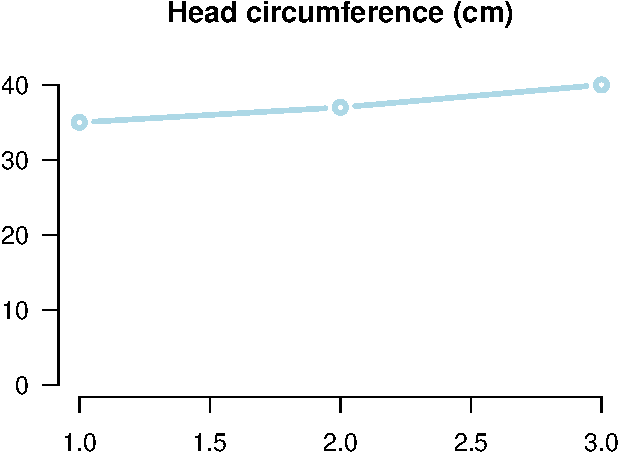
\includegraphics{eli_files/figure-latex/unnamed-chunk-11-1.pdf}

\paragraph{Weight}\label{weight}

\begin{Shaded}
\begin{Highlighting}[]
\NormalTok{wv <-}\StringTok{ }\KeywordTok{gsub}\NormalTok{(}\StringTok{"[^[:digit:]]"}\NormalTok{, }\StringTok{""}\NormalTok{, weight}\OperatorTok{$}\NormalTok{Value) }\CommentTok{# get just integers}
\KeywordTok{stri_sub}\NormalTok{(wv,}\DecValTok{2}\NormalTok{) <-}\StringTok{ "."} \CommentTok{# insert the decimal point in the correct place}
\NormalTok{weight}\OperatorTok{$}\NormalTok{Value <-}\StringTok{ }\NormalTok{wv }\OperatorTok\StringTok{ }\KeywordTok{as.numeric}\NormalTok{() }\CommentTok{# make numeric}

\KeywordTok{par}\NormalTok{(}\DataTypeTok{las=}\DecValTok{1}\NormalTok{,}\DataTypeTok{bty=}\StringTok{"n"}\NormalTok{)}
\NormalTok{ylim <-}\StringTok{ }\KeywordTok{round}\NormalTok{(}\KeywordTok{max}\NormalTok{(weight}\OperatorTok{$}\NormalTok{Value,}\DecValTok{10}\NormalTok{))}
\KeywordTok{with}\NormalTok{(weight,}\KeywordTok{plot}\NormalTok{(Value,}
                 \DataTypeTok{col=}\StringTok{"pink"}\NormalTok{,}\DataTypeTok{type=}\StringTok{"b"}\NormalTok{,}\DataTypeTok{lwd=}\DecValTok{3}\NormalTok{,}
                 \DataTypeTok{ylim=}\KeywordTok{c}\NormalTok{(}\DecValTok{0}\NormalTok{,ylim)}
\NormalTok{))}
\KeywordTok{axis}\NormalTok{(}\DecValTok{1}\NormalTok{,}\DataTypeTok{xlab=}\NormalTok{month.name[}\KeywordTok{length}\NormalTok{(head}\OperatorTok{$}\NormalTok{Value)])}
\KeywordTok{title}\NormalTok{(}\StringTok{"Weight (g)"}\NormalTok{)}
\end{Highlighting}
\end{Shaded}

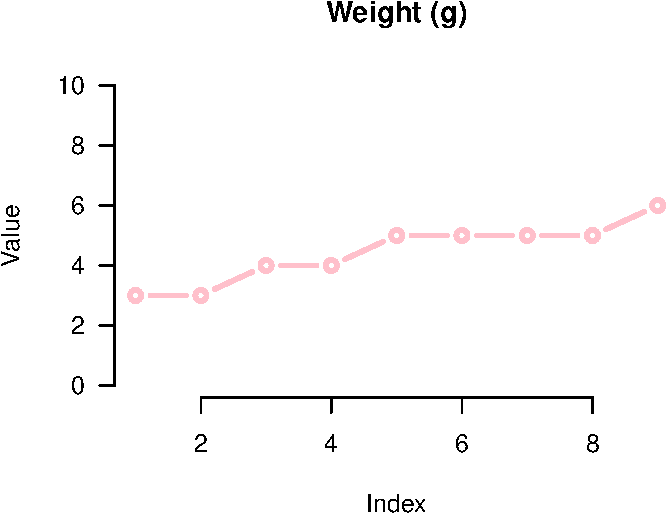
\includegraphics{eli_files/figure-latex/unnamed-chunk-12-1.pdf}

\paragraph{Height}\label{height}

\begin{Shaded}
\begin{Highlighting}[]
\NormalTok{hhv <-}\StringTok{ }\KeywordTok{gsub}\NormalTok{(}\StringTok{"[^[:digit:]]"}\NormalTok{, }\StringTok{""}\NormalTok{, height}\OperatorTok{$}\NormalTok{Value) }\CommentTok{# get just integers}
\KeywordTok{stri_sub}\NormalTok{(hhv,}\DecValTok{3}\NormalTok{) <-}\StringTok{ "."}\NormalTok{ ;hhv }\CommentTok{# insert the decimal point in the correct place}
\end{Highlighting}
\end{Shaded}

\begin{verbatim}
[1] "53." "55." "61." "63."
\end{verbatim}

\begin{Shaded}
\begin{Highlighting}[]
\NormalTok{height}\OperatorTok{$}\NormalTok{Value <-}\StringTok{ }\NormalTok{hhv }\OperatorTok\StringTok{ }\KeywordTok{as.numeric}\NormalTok{() }\CommentTok{# make numeric}

\KeywordTok{par}\NormalTok{(}\DataTypeTok{las=}\DecValTok{1}\NormalTok{,}\DataTypeTok{bty=}\StringTok{"n"}\NormalTok{)}
\KeywordTok{with}\NormalTok{(height,}\KeywordTok{plot}\NormalTok{(Value,}
                 \DataTypeTok{col=}\StringTok{"pink"}\NormalTok{,}\DataTypeTok{type=}\StringTok{"b"}\NormalTok{,}\DataTypeTok{lwd=}\DecValTok{3}\NormalTok{,}
                 \DataTypeTok{ylim=}\KeywordTok{c}\NormalTok{(}\DecValTok{0}\NormalTok{,}\DecValTok{70}\NormalTok{)}
\NormalTok{))}
\CommentTok{# axis(1,xlab=month.name[length(head$Value)])}
\KeywordTok{title}\NormalTok{(}\StringTok{"Height (cm)"}\NormalTok{)}
\end{Highlighting}
\end{Shaded}

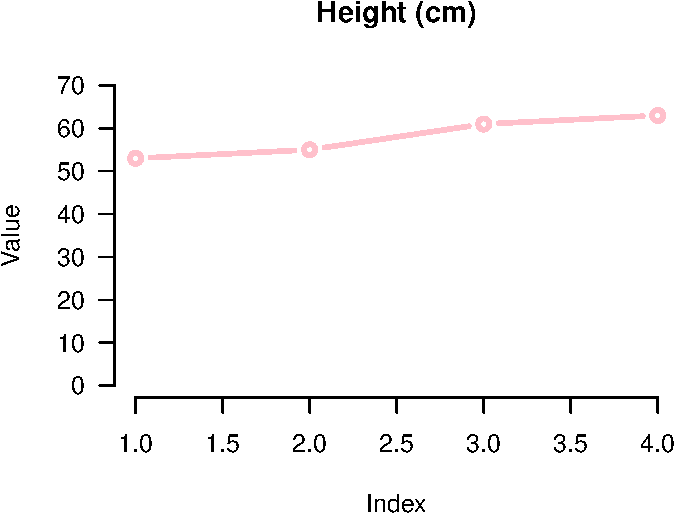
\includegraphics{eli_files/figure-latex/unnamed-chunk-13-1.pdf}

\subsubsection{Feeding}\label{feeding}

\paragraph{Left breast}\label{left-breast}

\paragraph{Right breast}\label{right-breast}

\subsubsection{Diaper}\label{diaper}

\begin{Shaded}
\begin{Highlighting}[]
\KeywordTok{unique}\NormalTok{(diaper}\OperatorTok{$}\NormalTok{Trait)}
\end{Highlighting}
\end{Shaded}

\begin{verbatim}
[1] "Pee & Poo" "Poo"       "Pee"      
\end{verbatim}

\paragraph{Pee}\label{pee}

\begin{Shaded}
\begin{Highlighting}[]
\KeywordTok{unique}\NormalTok{(diaper}\OperatorTok{$}\NormalTok{Trait)}
\end{Highlighting}
\end{Shaded}

\begin{verbatim}
[1] "Pee & Poo" "Poo"       "Pee"      
\end{verbatim}

\paragraph{Poo}\label{poo}

\begin{Shaded}
\begin{Highlighting}[]
\KeywordTok{unique}\NormalTok{(diaper}\OperatorTok{$}\NormalTok{Trait)}
\end{Highlighting}
\end{Shaded}

\begin{verbatim}
[1] "Pee & Poo" "Poo"       "Pee"      
\end{verbatim}

\paragraph{Both}\label{both}

\begin{Shaded}
\begin{Highlighting}[]
\KeywordTok{unique}\NormalTok{(diaper}\OperatorTok{$}\NormalTok{Trait)}
\end{Highlighting}
\end{Shaded}

\begin{verbatim}
[1] "Pee & Poo" "Poo"       "Pee"      
\end{verbatim}

\subsubsection{Leisure}\label{leisure}

\paragraph{Bath}\label{bath}

\paragraph{Tummy}\label{tummy}

\paragraph{Outdoors}\label{outdoors}

\paragraph{Play}\label{play}

\subsubsection{Lab}\label{lab}

\printbibliography

\end{document}
